\chapter{Subpatterns}\indexmain{subpatterns}
\label{cha:sub}

After the introduction of the nested patterns in chapter \ref{cha:nested} we will now have a look at the subpatterns, the other means to greatly enhances the flexibility and expressiveness of pattern matching and rewriting.
Subpattern employment is split into subpattern declaration plus subpattern entity declaration, and subrule declaration plus usage, the latter is described in the following chapter.

%%%%%%%%%%%%%%%%%%%%%%%%%%%%%%%%%%%%%%%%%%%%%%%%%%%%%%%%%%%%%%%%%%%%%%%%%%%%%%%%%%%%%%%%%%%%%%%%
\section{Subpattern Declaration}
\indexmain{subpattern}\label{sec:subpattern}

Subpatterns were introduced to factor out a common recurring pattern -- a shape -- into a named subpattern type, ready to be reused at points the pattern should get matched.
The common recurring pattern is specified in a subpattern declaration and used by a subpattern entity declaration.

\begin{rail}  
  SubpatternDeclaration: 
    'pattern' IdentDecl Parameters? (('modify'|'replace') Parameters)? \\
	lbrace SubpatternBody rbrace ;
  SubpatternBody: (PatternStatement+) SubpatternRewriting?;
\end{rail}\ixkeyw{pattern}\ixkeyw{modify}\ixkeyw{replace}\ixnterm{SubpatternDeclaration}\ixnterm{SubpatternBody}\label{subpatterndecl}\indexmain{subpattern declaration}

Subpattern declarations define a subpattern type denoting the specified shape in the global namespace;
the parameters specify some context elements the pattern may refer to, but which are not part of the pattern itself. 

So they are only syntactically the same as test/rule-parameters (which are members of the pattern part).
A further difference is the lack of \emph{ReturnTypes}; they are not actions, just a helper in constructing complex patterns.
In order to get values out they employ the language construct of def entities which are yielded to (cf. \ref{cha:yielding}).
Subpatterns can receive additional rewrite parameters, in addition to the pattern parameters, and in contrast to the actions; they can be used to hand in nodes which are created in the rewrite part of the action or subpattern which contains the subpattern entity.
They apply to the nested subpattern rewriting part, which will be explained in Section~\ref{sec:subrule}.

\section{Subpattern Entity Declaration}

\begin{rail}  
  SubpatternEntityDeclaration: 
    Ident ':' SubpatternType '(' ((Ident|Expression) * ',') ')' ';' ;
\end{rail}\ixnterm{SubpatternEntityDeclaration}\indexmain{subpattern entity declaration}

Subpattern entity declarations (subpattern usages) instantiate an entity of the subpattern type (i.e. specified shape), which means the subpattern must get matched for the matching of the enclosing pattern to succeed.
The arguments given are bound to the corresponding parameters of the subpattern.
If you prefer a syntactical point of view, you may see the subpattern entity as a placeholder, which gets substituted in place by the textual body of the subpattern declaration under renaming of the parameters to the arguments.
If you prefer an operational point of view, you may see the subpattern entity as a call to the matcher routine searching for the specified pattern from the given arguments on (constructing a match piece, which is the base for rewriting of that part).

%TODO:remove
%Termersetzung mit Termen die Graphen beschreiben.
%Mehrelementige Graphsprachen als Zwischenschritt zu den rekursiven bereits mit alternative... eingef�hrt -- dort auch so erkl�rt, wirklich eingef�hrt? vor rekursiv trotzdem noch ein  Zwischenschritt: pattern mit alternative, statt action mit alternative

\begin{example}
  \begin{grgen}
pattern TwoParameters(mp:Method)
{
  mp <-- :Variable;
  mp <-- :Variable;
}
test methodAndFurther
{
  m:Method <-- n:Name;
  tp:TwoParameters(m);
}
  \end{grgen}

  In the given example a subpattern \texttt{TwoParameters} is declared, connecting the context element \texttt{mp} via two edges to two variable nodes.
  The test \texttt{methodAndFurther} is using the subpattern via the declaration of the entity \texttt{tp} of type \texttt{TwoParameters}, binding the context element to its local node \texttt{m}.
  The resulting test after subpattern derivation is equivalent to the test \texttt{methodWithTwoParameters}.

  \begin{grgen}
test methodWithTwoParameters
{
  m:Method <-- n:Name;
  m <-- :Variable;
  m <-- :Variable;
}
  \end{grgen}
\end{example}

%-----------------------------------------------------------------------------------------------
\subsection{Recursive Patterns}\indexmain{recursive pattern}\indexmain{structural recursion}

Subpatterns can be combined with alternative patterns or the cardinality patterns into recursive subpatterns, i.e. subpatterns which may contain themselves.
Subpatterns containing themselves alone -- directly or indirectly -- would never yield a match as an infinite pattern can't be found in a limited graph.

\begin{example}\label{exiterpath}
  \begin{grgen}
test iteratedPath
{
  root:Assign;
  negative { --> root; }
  :IteratedPath(root); // match iterated path = assignment list
}

pattern IteratedPath(prev:Node)
{
  optional { // nothing or a linked assignment and again a list
    prev --> a:Assign; // assignment node 
    :IteratedPath(a); // next one, plz
  }
}
  \end{grgen}
  
The code above searches an \indexed{iterated path} from the root node on, here an assignment list. 
The iterated \indexed{path} with the optional is equivalent to the code below. Note the negative which ensures you get a longest match -- without it the empty case may be chosen lazily just in the beginning.
Please note that if you only need to check for the existence of such a simple iterated path you can use the \texttt{reachable} functions, or even better \texttt{isReachable} predicates introduced in \ref{transitiveneighbour}.

  \begin{grgen}
pattern IteratedPath(prev:Node)
{
  alternative {
    Empty {
      negative {
        prev --> a:Assign;
      }
    }
    Further {
      prev --> a:Assign;
      :IteratedPath(a);
    }
  }
}
  \end{grgen}

The code below searches an iterated path like the code above, just that it stops when a maximum length is reached.
The \indexed{bounded iterated path} is realized by 
calling a pattern with the requested maximum depth,
counting the depth parameter down with each recursion step,
until the limit checked by a condition is reached.
The \texttt{boundedReachable} functions introduced in \ref{transitiveneighbourbounded} should be preferred in a simple case like this.

  \begin{grgen}
test boundedIteratedPath(root:Assign)
{
  :BoundedIteratedPath(root, 3); // match iterated path of depth 3
}

pattern BoundedIteratedPath(prev:Node, var depth:int)
{
  optional { // nothing or a linked assignment and again a list
    prev --> a:Assign; // assignment node 
    :IteratedPath(a, depth-1); // next one, plz
    if{ depth >= 1; } // stop when we have reached max depth
  }
}
  \end{grgen}
\end{example}

\begin{example}
  \begin{grgen}
rule removeMiddleAssignment
{
  a1:Assign --> a2:Assign --> a3:Assign;
  independent {
    :IteratedPath(a1,a3)
  }
  
  replace {
    a1; a3;
  }
}

pattern IteratedPath(begin:Assign, end:Assign)
{
  alternative { // an iterated path from begin to end is either
    Found { // the begin assignment directly linked to the end assignment (base case)
      begin --> end;
    }
    Further { // or an iterated path from the node after begin to end (recursive case)
      begin --> intermediate:Assign;
      :IteratedPath(intermediate, end);
    }
  }
}
  \end{grgen}

This is once more a fabricated example, for an iterated path from a source node to a distinctive target node, and an example for the interplay of subpatterns and positive application conditions to check complex conditions independent from the pattern already matched.
Here, three nodes \texttt{a1},\texttt{a2},\texttt{a3} of type \texttt{Assign} forming a list connected by edges are searched, and if found, \texttt{a2} gets deleted, but only if there is an iterated path of directed edges from \texttt{a1} to \texttt{a3}.
The path may contain the host graph node matched to \texttt{a2} again.
Without the \texttt{independent} this would not be possible, as all pattern elements -- including the ones originating from subpatterns -- get matched isomorphically. 
The same path specified in the pattern of the rule -- not in the independent -- would not get matched if it would go through the host graph node matched to b, as it is locked by the isomorphy constraint.
Again, the \texttt{reachable} functions and \texttt{isReachable} predicates introduced in \ref{transitiveneighbour} are the better choice here.
They always match independently from the patterns (so when you need locking, you cannot employ them), can be used directly, and are implemented (more) efficiently. 
\end{example}

With recursive subpatterns you can already capture neatly structures extending into depth (as iterated paths)
and also structures extending into breadth (as forking patterns, although the cardinality statements are often much better suited to this task).
But combined with an iterated block, you may even match structures extending into breadth and depth,
like e.g. an inheritance hierarchy of classes in our example domain of program graphs, see example \ref{exsptree}, i.e. you can match a \indexed{spanning tree} in the graph.
This gives you a very powerful and flexible notation to capture large, complex patterns
built up in a structured way from simple, connected pieces (as e.g. abstract syntax trees of programming languages). 

\begin{note}
If you are working with hierarchic structures like that, 
you might be interested in the capabilities of GrShell/yComp for nested layout
as described and shown in \ref{sub:visual}/\ref{note:visual}).
\end{note}

\begin{example}\label{exsptree}
  \begin{grgen}
pattern SpanningTree(root:Class)
{
  iterated {
    root <-:extending- next:Class;
    :SpanningTree(next);
  }
}
  \end{grgen}
\end{example}

\begin{example}

\begin{center}
  \parbox{0.99\linewidth}{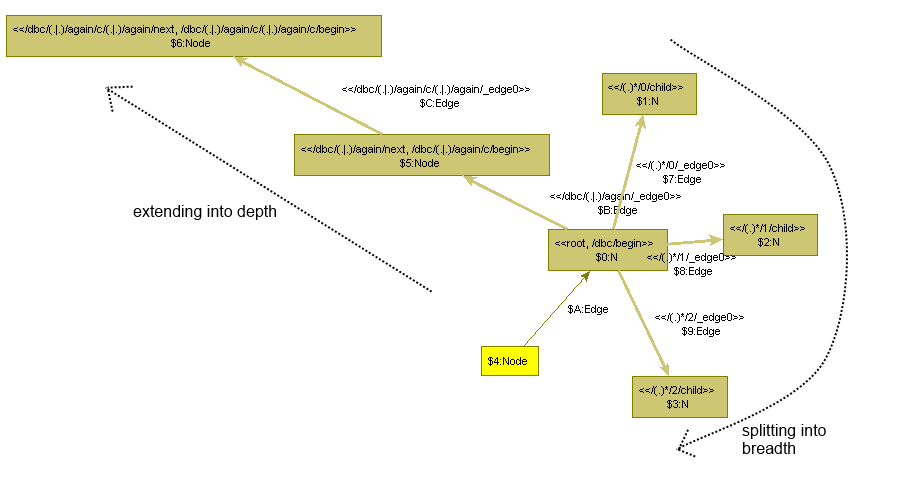
\includegraphics[width=\linewidth]{fig/exdepthbreadth}}
\end{center}

The image from above visualizes the matching of structures extending into depth and splitting into breadth, employing the pattern of test \texttt{db} from below.

\begin{grgen}
test db(root:Node)
{
  iterated {
    root --> child:N;
  }	
  dbc:chain(root);
}
pattern chain(begin:Node)
{
  alternative {
    again {
      begin --> next:Node;
      c:chain(next);
    }
    end {
      negative { begin --> .; }
    }
  }
}
\end{grgen}

\end{example}

\begin{example}

The example from the previous page utilizes the nested and subpatterns introduced in this and the previous chapter;
it matches \texttt{db} from a \texttt{root} node handed in on, in a tiny example graph (built from nodes of types \texttt{Node} and \texttt{N}, and edges of type \texttt{Edge}). 

The breadth-splitting structure is collected with an \texttt{iterated} pattern around the center node bound to the pattern node \texttt{root}.
The graph elements are annotated in the debugger (cf. Chapter~\ref{chapdebugger}) as usual with their pattern element name -- plus the (sub)pattern nesting path that lead to the instance of this pattern.

The \verb#(.)*/1/child# at the middle-right node tells that the node is contained in an iterated pattern (using the regular expression syntax for the iterated, see Table~\ref{keywordregexpsyntax}), that this is instance \texttt{1} (starting at \texttt{0}, here we got 3 matches of the iterated, so ending at instance count \texttt{2}, and that the name of the element in the pattern is \texttt{child}.

The depth-extending structure is collected with a subpattern \texttt{chain} employed from the test with the instance \texttt{dbc} starting at the node bound to the pattern node \texttt{root}.
It uses itself recursively with the subpattern instance \texttt{c}, from the node \texttt{next} on, which is reached with one edge-following-step from the input node \texttt{begin} on.

The \verb#/dbc/(.|.)/again/next# at the middle node of the chain tells that the node was matched on the subpattern instance named \texttt{dbc}, in an alternative (using regular expression syntax for the alternative), in the pattern of the \texttt{again} case, to the pattern node named \texttt{next}.
The same node is annotated with an\verb#/dbc/(.|.)/again/c/begin#, which stems from the fact that the node appears also in the next nesting step (subpattern call), in the instance \texttt{c} of the subpattern instantiated in the branch \texttt{again}; as \texttt{begin} node handed in to \texttt{chain}.

Breadth-splitting structure-matching is typically following \texttt{contains} edges, while depth-extending structure-matching is typically following \texttt{next} edges, please take a look at the Hints on Modeling~\ref{modelcontainsnext}. 

The (sub)pattern nesting paths can get long, cluttering display, so from a certain size on, only the size of the path is printed in the debugger. 

\end{example}


%%%%%%%%%%%%%%%%%%%%%%%%%%%%%%%%%%%%%%%%%%%%%%%%%%%%%%%%%%%%%%%%%%%%%%%%%%%%%%%%%%%%%%%%%%%%%%%%
\section{Regular Expression Syntax}\indexmainsee{EBNF}{regular expression syntax}\indexmain{regular expression syntax}

In addition to the already introduced syntax for the nested patterns with the keywords 
\texttt{negative}, \texttt{independent}, \texttt{alternative}, \texttt{iterated}, \texttt{multiple} and \texttt{optional},
there is a more lightweight syntax resembling regular expressions available; 
when used together with the subpatterns it yields graph rewrite specifications which look like EBNF-grammars with embedded actions. 
Besides reducing syntactical weight, they offer constructs for matching a pattern a bounded number of times (same notation as the one for the bounded iteration in the sequences).

%Table \ref{keywordregexpsyntax} lists the corresponding (/equivalent) language constructs; 
%Example \ref{introexampleregexp} is a version of the introductory example \ref{introexample} modified to use the new syntax. commented out to get better layout

\begin{table}[htbp]
  \centering
  \begin{tabularx}{\linewidth}{|l|X|} \hline
    \texttt{ iterated \{ P \} } & \texttt{ (P)* } \\
    \texttt{ multiple \{ P \} } & \texttt{ (P)+ } \\
    \texttt{ optional \{ P \} } & \texttt{ (P)? } \\ 
	\texttt{ alternative \{ l1 \{ P1 \} .. lk \{ Pk \} \} } & \texttt{ (P1|..|Pk) } \\
    \texttt{ negative \{ P \} } & \texttt{ $\sim$(P) } \\
    \texttt{ independent \{ P \} } & \texttt{ \&(P)} \\ \hline 
    \texttt{ modify \{ R \} } & \texttt{  \{+ R \} } \\
    \texttt{ replace \{ R \} } & \texttt{ \{- R \} } \\ \hline 
    \texttt{ - } & \texttt{ (P)[k] / (P)[k:l] / (P)[k:*] } \\ \hline 
	\end{tabularx}
  \caption{Map of nested patterns in keyword syntax to regular expression syntax}
  \label{keywordregexpsyntax}
\end{table}

Understanding \GrG-subpatterns may be easier given knowledge about EBNF-grammars when we compare them to those.
We find then that rules resemble grammar axioms, subpatterns resemble nonterminals, and graphlets resemble terminal symbols; nested patterns are similar to EBNF operators, and the rewrite part corresponds to the semantic actions of syntax directed translation.
Negative and independent patterns are used to explicitly check context constraints
(every graphlet as such is already able to match pieces that one would or could classify as context, graph rewriting allows for derivations that are highly adaptable to the surrounding parts).
See \cite{EBNFAGTIVE} for more on this.

  \begin{example}
    \begin{grgen}
test method
{
  m:Method <-- n:Name; // signature of method consisting of name
  ( m <-- :Variable; )* // and 0-n parameters
  
  :AssignmentList(m); // body consisting of a list of assignment statements
}

pattern AssignmentList(prev:Node)
{
  ( // nothing or a linked assignment and again a list
    prev --> a:Assign; // assignment node 
    a -:target-> v:Variable; // which has a variable as target 
    :Expression(a);  // and an expression which defines the left hand side 
    :AssignmentList(a); // next one, plz
  )?
}

pattern Expression(root:Expr)
{
  ( // expression may be a binary expression of an operator and two expresions
      root <-- expr1:Expr;
      :Expression(expr1);
      root <-- expr2:Expr;
      :Expression(expr2);
      root <-- :Operator;
  | // or a unary expression which is a variable (reading it)
      root <-- v:Variable;
  )
}
    \end{grgen}
  \end{example}\label{introexampleregexp}

%%%%%%%%%%%%%%%%%%%%%%%%%%%%%%%%%%%%%%%%%%%%%%%%%%%%%%%%%%%%%%%%%%%%%%%%%%%%%%%%%%%%%%%%%%%%%%%%
\section{Locking}\label{locking}

\subsubsection*{Isomorphy Locking}
When matching a program graph as in the introductory example \ref{ex:proggraph} one might be satisfied with matching a tree structure.
But on other occasions one wants to match \emph{backlinks} and especially the targets of the backlinks, too, 
from \emph{uses} nested somewhere in the syntax graph to \emph{definitions} whose nodes were already matched earlier in the subpattern derivation (subpatterns can be seen as an equivalent of grammar rules known from parser generators).
Unfortunately these elements are already matched and thus isormorphy locked following the default semantics of isomorphic matching.
And unfortunately these elements can't be declared \texttt{hom}omorphic as they are unknown in the nested subpattern.
Handing them in as parameters and then declaring them \texttt{hom}omorphic is only possible if they are of a statically fixed number (as the number of parameters is fixed at compile time), which is normally not the case for e.g. the attributes of a class in a syntax graph.
In order to handle this case the \texttt{independent} \emph{operator} (cf. \ref{rule:homspec}) was added to the rule language
--- when you declare the backlink target node \texttt{n} as \texttt{independent(n)} it can be matched once again.
Thus it is possible to match e.g. a class attribute definition node which was already matched when collecting the attributes of the class again later on in a subpattern when matching an expression containing a usage of that attribute, allowing to e.g. add further edges to it.

\subsubsection*{Patternpath Locking} 
As stated in the sections on the negative and independent constructs (\ref{nac}, \ref{pac}), they get matched homomorphically to all already matched elements. By referencing an element from outside you can isomorphy lock that element to prevent it to get matched again.

Maybe you want to lock all elements from the directly enclosing pattern, in this case you can just insert \texttt{pattern;} in the position of a graphlet into the NAC or PAC.

Maybe you want to lock all elements from the patterns dynamically containing the NAC/PAC of interest, i.e. all subpattern usages and nesting patterns on the path leading to the NAC/PAC of interest (but not their siblings). In this case you can insert \texttt{patternpath;} in the position of a graphlet into the NAC or PAC. You might be interested in this construct when matching a piecewise constructed pattern, e.g. a chain, which requires to check for another chain (iterated path) which is not allowed to cross (include an element of) the original one.


%todo: quick reference table showing a pattern one is interested in and the language construct to capture it (breadth, alternativem, depth, ..)
